%!TEX root = ../master.tex
\section{Cryptography}
This section will briefly introduce concepts from cryptography relevant to the project, and will be based on \cite{cryptoenginerring}.

\subsection{Terms}
Alice
Bob 
Eve


\subsection{Encryption}

\subsection{Authentication}
When Alice sends messages to Bob over some insecure channel it can be possible for Eve to change how Bob recieves the messages.
Eve can alter the sent message \emph{m} to \emph{m'} and send \emph{m'} to Bob without Bob knowing.
Eve can also change the order of messages so a message comes much later than intended.
If Eve delete a message Bob will never know that this message existed.
Eve can even create her own message and send it without Bob can know that this message was not created by Alice.

The solution to these problems is authentication of messages.
Alice and Bob have a shared secret key $K_a$ for authentication.

\begin{figure}[tb]
	\centering
	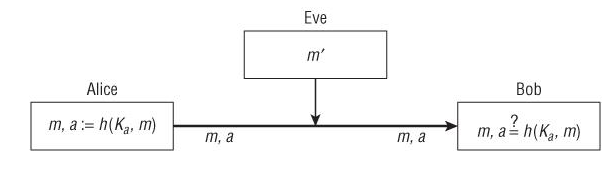
\includegraphics[width=\textwidth]{authenticationSetup}
	\caption{Setup for authentication. From \citet{cryptoenginerring}
	\label{crypto:authsetup}
\end{figure}

